\chapter{Virtualization}

\section{Segmentation And Paging}

\subsection{Segmentation}

    Segmentation is compiler's view about memory.

    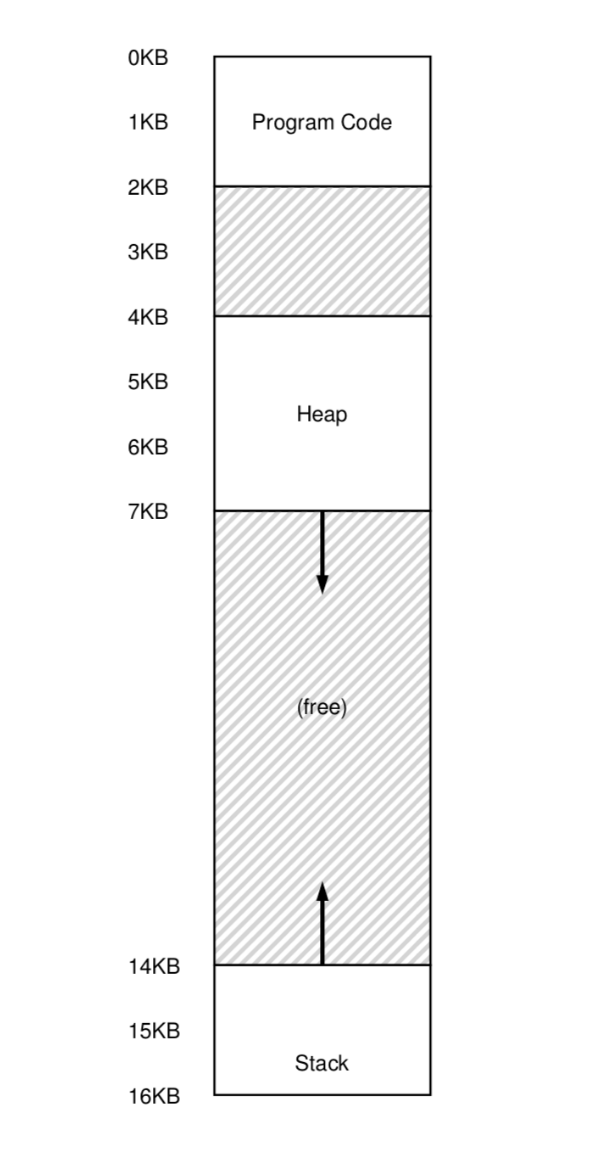
\includegraphics[width=0.45\textwidth]{chapters/chapter1/Segmentation_Paging/Segmentation.png}

    In canonical address space, we have three logically-different segments:
    \begin{enumerate}
        \item Code/Text
        \item Heap
        \item Stack
    \end{enumerate}

\sssc{Base/Bound registers}
    Each segments would have a pair of base and bound registers.

    We would use base and bound/limit registers to translate address. 
    
    \begin{center}
        Physical Address = Base Address + Offset
    \end{center}

    Bound register is used to check boundary. If offset is greater than
    bound register value $\Rightarrow$ Segmentation fault.

    \textit{Note: the stack grows in opposite direction}
\sssc{Referring Segments}

    We would chop up the address space into two parts:

    \begin{enumerate}
        \item 2 bits: indicate the segments
        \item the reset: offset within the segments
    \end{enumerate}

    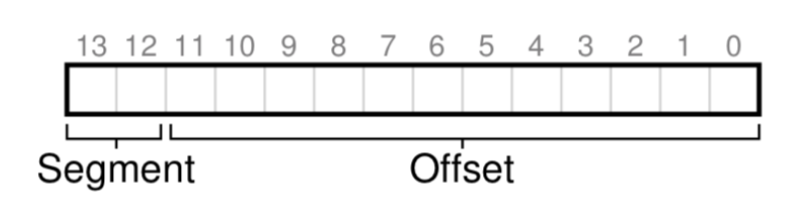
\includegraphics[width=0.45\textwidth]{chapters/chapter1/Segmentation_Paging/ReferingSegments.png}

    Assume 8-bit address space in use:
    \begin{enumerate}
        \item 00xxxxxx: this is invalid, we would address 1/4 less because we don't use 00. 
        \item 01xxxxxx: would be in the Code segment.
        \item 10xxxxxx: would be in the Heap segment.
        \item 11xxxxxx: would be in the Stack segment.
    \end{enumerate}

\sssc{Support for sharing}

    It is good idea to share the code segment, but how the OS supports it?

    There would be protection bits to indicate whether the segment can be used for.
    
    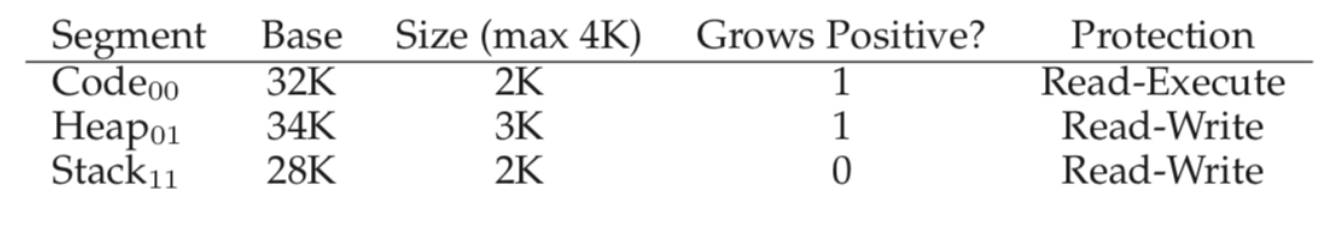
\includegraphics[width=0.45\textwidth]{chapters/chapter1/Segmentation_Paging/SegementWithProtection.png}

\sssc{OS support}

    So support segmentation, the OS
    \begin{enumerate}
        \item Context Switch: The segment registers must be saved and restored.
        \item Support growth or shrinkage of a segment: Management of free space, Compacting physical memory and
        Free-list management algorithms.
    \end{enumerate}

\subsection{Free Space Management}

\sssc{Low-level Mechanisms}

    Spliting and coalescing:

\sssc{Basic Strategies}


\subsection{Advanced Page Tables}


\section{Swapping}

   
\subsection{Swapping Mechanisms}

Use hard disk drive to stash portions of address spaces that currently aren't in
great demand, so that we can support programs that take more memories than RAM has.

\sssc{Swap Space}

    Swap Space: Reserved space on the disk for moving pages back and forth.

    And OS can read from and write to swap space in page-sized units. Also OS needs
    to know the exact address of the swap space inorder to quickly swap pages.

\sssc{The Present Bit}  

    Inside of page table entry, there is a present bit.

    When the present bit is set, that indicates the page is in the physical memory.

    It the present bit is off, the page in not in the memory. When a TLB miss resulting
    in a page table entry and found the present bit is off, it is a page fault (indicates
     the demanding page is not in the physical memory).

\sssc{The Page Fault}

    The OS would invokes Page-Fault Handler to deal with page fault.
    
    \begin{enumerate}
        \item The OS would look into PTE(page table entry) to find the address to fetch.
        \item After completing disk I/O, the OS updates PTE to mark the page as present.
        \item Update the PFN(physical frame number) of the PTE to the in-memory location
        of the fetched-page.
        \item Retry the instruction.
    \end{enumerate}

\sssc{When the memory is full}

    When page-fault and the memory is full, the OS needs to kick out a page to place
    a new page in. Therefore, page-replacement policy is needed.

\subsection{Swapping Policies}

\sssc{Cache Management}

    Main memory holds some subset of all the pages of ongoing processes  $\Rightarrow$
    main memory is a cache for virtual memory pages.

    The goal is to minimize the number of cache misses.

    \textbf{Average Memory Access Time}
    \begin{equation*}
        AMAT = T_M + (P_{miss}\times T_D)
    \end{equation*}
    Where,
    \begin{enumerate}
        \item $T_M$: the cost of accessing memory
        \item $T_D$: the cost of accessing disk
        \item $P_miss$: the probability of cache miss
    \end{enumerate}

    Assume that $T_M$ = 100 nanoseconds, $T_D$ = 10 milliseconds .
    
    If the hit rate is 0.9, the AMTA would be 100ns + 0.1 · 10ms = 1.0001 ms.

    However, when the hit rate is 0.99, the AMTA would be 10.01 microsecs which is 
    100x faster. That is, the perfomance is heavily based on the hit rate $\rightleftarrows$
    swapping policy matters.

\sssc{The Optimal Replacement Policy}

    The optimal replacement policy leads to the fewest number of misses overall.

    Belady (a person) showed that a simple policy that leads to optimal:
    The page that would be accessed furthest in the future is the optimal policy
    (This is very like shortest job first CPU scheduling,i.e, impossible!)

    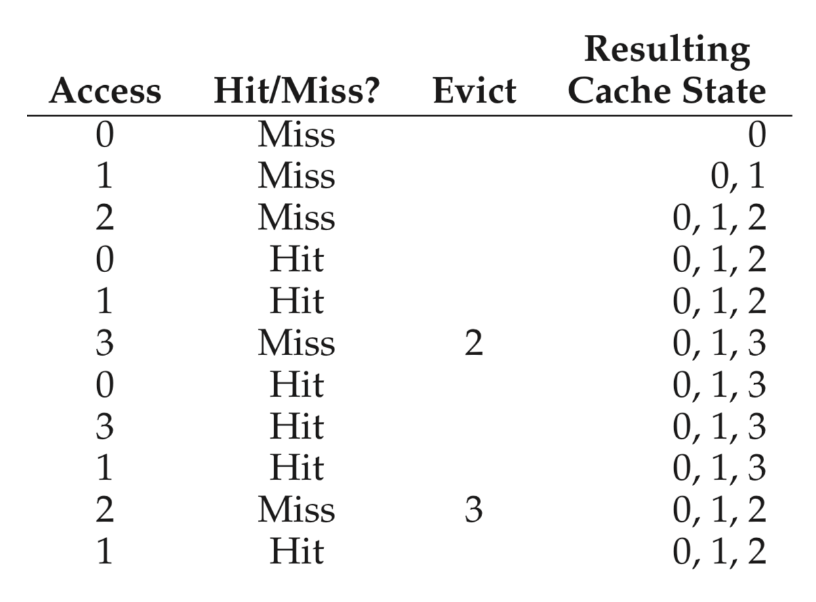
\includegraphics[width=0.45\textwidth]{chapters/chapter1/Segmentation_Paging/OptimalSwappingPolicy.png}

    First three accesses are misses, and the misses are called \textbf{cold-start misses}.

    When Access 3 at the first time, the optimal policy decides to evict 2 because
    0 and 1 would be accessed before 2.

    However, future is  unpredicable, an another approach is needed.

\sssc{FIFO}

    Old friend, First In First Out.

    FIFO is very simple to implement.

    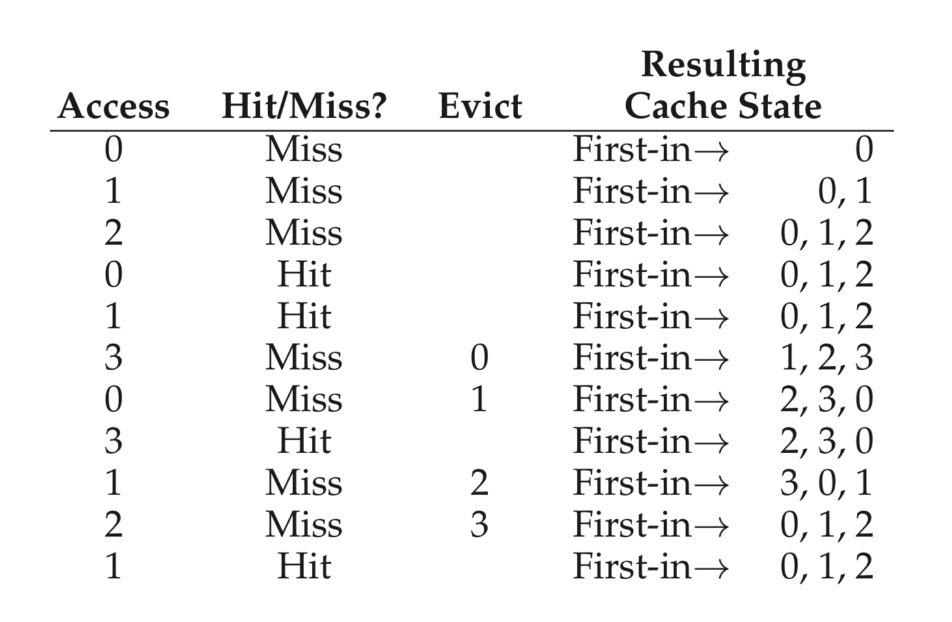
\includegraphics[width=0.45\textwidth]{chapters/chapter1/Segmentation_Paging/FIFO.png}

    FIFO could often do poorly because it cannot determine the importance of a page.


\sssc{Random}

    Simple to implement, and do well if the distribution of accessing page is uniform
    distributed. However, it is unlikely for accessing page to follow a particular
    distribtion.

    Random is better than FIFO, and a bit worst than optimal.

\sssc{LRU}

    If page is accessed in the near past, it is likely to be accesed in near future.

    Some historically-based algorithms are used. LFU: Least-Frequently-Used, and
    LRU: Least-Recently-Used.

    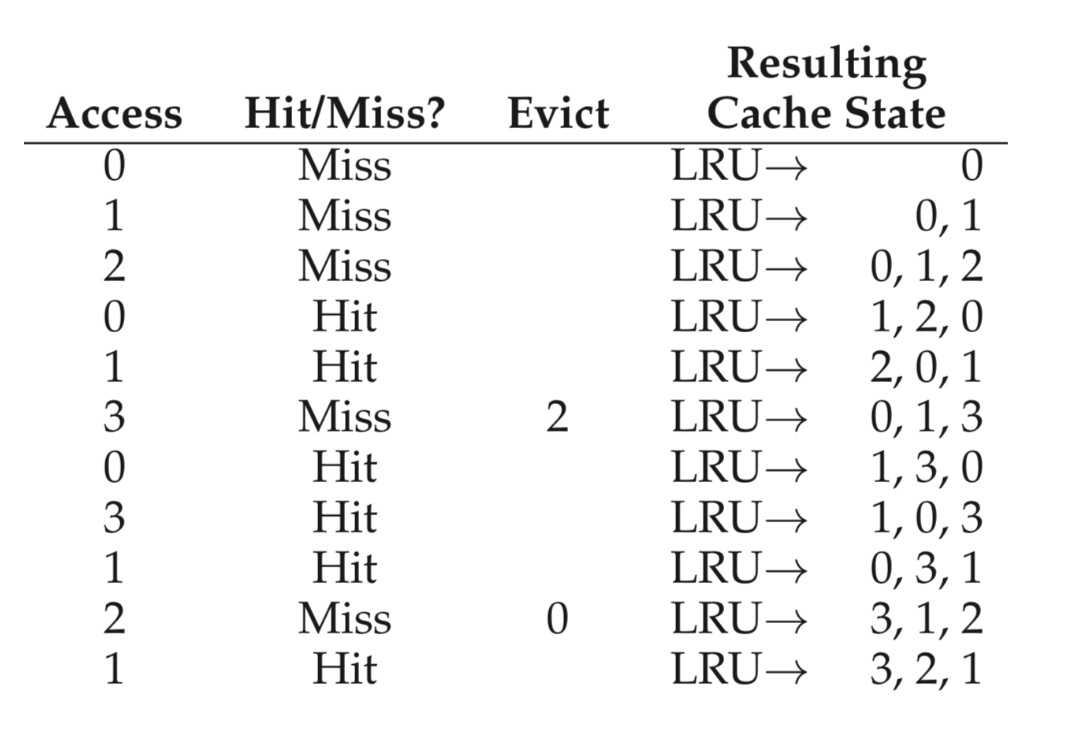
\includegraphics[width=0.45\textwidth]{chapters/chapter1/Segmentation_Paging/LRU.png}

    The LRU policy works well to matching the optimal.

\sssc{Implement Historical Algorithms}

    Using LRU, the system needs to count the least- and most-recently used which is 
    a lot of work. Bad implementation would led heavy performance penalty.

    Even adding timestamp for every process accessing, it is unlikely to scan the all
    pages to find the abosulte least recently used page.

    \tbi{Approximating LRU} would be a solution:
    \begin{enumerate}
        \item Need a \underline{use bit}: use bit is set to 1 when the page is accessed.
        \item Use a clock algorithm: a clock pointer points to each particular page,
        if the use bit is 1, the OS clear the use bit and the pointer points to the next page.
        If found a page with use bit 0, replace it. The worst case is looping through the entire
        set of pages for one circle.
    \end{enumerate}

\sssc{Dirty Pages}

    If a page is modified while in the memory, it is dirty. It would cost a lot to 
    evict dirty page since the page must be written to the disk first. Therefore, 
    most algorithms would favor to evict clean pages over dirty pages.

    To support the behavior, the hardware includes a \underline{modified bit}. The bit 
    is set when the page is modified and cleared when written to disk.

\sssc{Other Policies}

    Page selection policy determines when to bring a page into the memory. For most 
    pages, OS would use \tbi{demanding paging}, which means the OS brings the 
    page into memory when it is accessed. Or OS would predict which page would be 
    accessed in the future and bring it to the memory, this is called \tbi{prefetching}.

    Another policy determines how the OS writes pages out to disk.
    \tbi{Clustering} is a behavior that OS buffers the changes and write out to disk
    in one write.

\sssc{Thrashing}

    \tbi{Thrashing}: When the demanding of pages exceed the available physical memory,
    the system would constantly being paging.

    Linux would ran \tbi{out-of-memory killer} to choose some memory-intensive process
    and kill them.